%! TEX root = part4.tex
% the main TeX file which is intended to compile, :VimtexReload after adjustment
% :h vimtex-tex-root
\documentclass[../main.tex]{subfiles}
% \includeonlyframes{current}
% \setbeameroption{hide notes} % Only slides
% \setbeameroption{show only notes} % Only notes
\setbeameroption{show notes on second screen=right} % Both

\begin{document}


\begin{frame}[mytitle=standard,c,mybg=bglight3,light]

	\begin{center}
		\boldred{Dikumpulkan}  : Gambar Kerja Rencana Pondasi
	\end{center}

\end{frame}

\begin{frame}[mytitle=center,t,mycolor=digiPH_uniblue,light]\frametitle{Balok dalam Struktur Bangunan}

	\txt{digiPH_gray}{digiPH_darkblue}{Balok merupakan elemen struktural horizontal yang berfungsi untuk mendistribusikan beban dari lantai, atap, atau dinding ke kolom atau pondasi.}

	Balok bekerja terutama terhadap:

	\begin{itemize}
		\item Gaya lentur (bending)
		\item Gaya geser (shear)
	\end{itemize}

	\footnotesize Perencanaan balok sangat penting untuk menjaga kekuatan dan stabilitas bangunan. \normalsize
\end{frame}


\begin{frame}[mytitle=center,t,mycolor=digiPH_ocean,dark]\frametitle{Fungsi Balok}

	Fungsi utama balok dalam struktur bangunan:

	\begin{itemize}
		\item Mendistribusikan beban dari lantai, atap, dan dinding ke kolom.
		\item Menahan gaya lentur akibat beban vertikal maupun horizontal.
		\item Menghubungkan kolom dengan elemen struktural lainnya.
		\item Membantu menjaga kestabilan rangka struktur bangunan.
	\end{itemize}
\end{frame}


\begin{frame}[mytitle=standard,t,mycolor=digiPH_white,light]\frametitle{Klasifikasi Balok}

	\begin{columns}
		\begin{column}{0.5\textwidth}
			Dalam konstruksi bangunan, balok dapat diklasifikasikan menjadi:

			\begin{itemize}
				\item Balok Induk (Primary Beam)
				\item Balok Anak (Secondary Beam)
			\end{itemize}

			Kedua jenis balok ini bekerja bersama untuk mendistribusikan beban secara efisien dalam struktur bangunan.
		\end{column}
		\begin{column}{0.5\textwidth}
			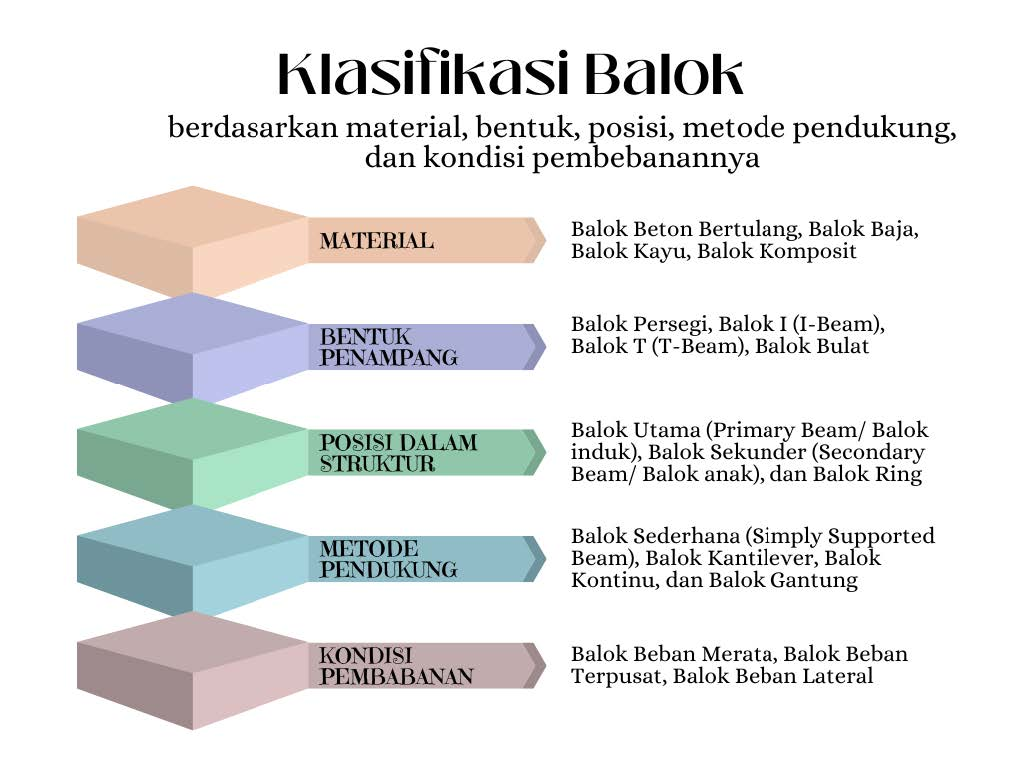
\includegraphics[width=.82\textwidth]{../figures/klasifikasi_balok.jpeg}
		\end{column}
	\end{columns}
\end{frame}

\begin{frame}[mytitle=standard,t,mycolor=digiPH_uniblue,light]\frametitle{Faktor yang Mempengaruhi Desain Balok}

	Beberapa faktor yang mempengaruhi perencanaan balok:

	\begin{itemize}
		\item Material yang digunakan:
		      \begin{itemize}
			      \item \item Beton bertulang
			      \item \item Baja
			      \item \item Kayu
		      \end{itemize}
		\item Beban yang dipikul
		\item Bentang (Span)
		\item[] Panjang balok mempengaruhi dimensi dan kekakuan balok.
		\item Jenis tumpuan
		\item Defleksi
		\item[] Untuk mencegah terjadinya deformasi berlebihan.
	\end{itemize}
\end{frame}

\begin{frame}[mytitle=standard,t,mycolor=digiPH_ocean,dark]
	\frametitle{Balok Induk (Primary Beam)}

	\txt{digiPH_ocean}{digiPH_white}{Balok induk adalah balok utama yang menerima beban dari:}

	\begin{itemize}
		\item Balok anak
		\item Lantai
		\item Dinding
	\end{itemize}

	Beban tersebut kemudian \boldred{diteruskan}  ke kolom.\end{frame}


\begin{frame}[mytitle=standard,c,mybg=bglight2,light]
	\frametitle{Perkiraan Dimensi Balok Induk}

	\only<1>{Dimensi balok induk biasanya ditentukan sekitar:

		\txt{digiPH_ocean}{digiPH_white}{1/10 – 1/20 dari bentang balok}
		\footnotesize}

	\only<2>{Contoh:

		Bentang = 600 cm

		Perhitungan:

		Lebar
		= 1/20 × 600
		= 30 cm

		Tinggi
		= 1/10 × 600
		= 60 cm

		\normalsize

		Dimensi balok induk ≈ 30 cm × 60 cm}
\end{frame}


\begin{frame}[mytitle=center,t,mycolor=digiPH_gray,light]
	\frametitle{Tugas Kelas (Lanjutan)}
	\txt{digiPH_leaf}{digiPH_white}{Buatlah maket Sloof dan Kolom berdasarkan denah yang tersedia.}
	\footnotesize Kelompok

\end{frame}

\begin{frame}[mytitle=center,t,mycolor=digiPH_gray,light]
	\frametitle{Tugas Rumah (Lanjutan)}
	\txt{digiPH_leaf}{digiPH_white}{Buatlah maket Balok berdasarkan denah yang tersedia.}

	\footnotesize Kelompok

	Buatlah Gambar Kerja \Huge Rencana Sloof dan Rencana Kolom \normalsize

	\footnotesize Individu

\end{frame}




\end{document}



